\qquad
为了充分验证本次实验中Wireshark软件真的抓到了登录过程中客户端向服务端提交的表单,下面将对捕获到的分组中TLS协议应用数据层的内容进行解密,以得到表单明文。完成解密后的分组如图 \ref{fig12} 所示。其中,标记为绿色,协议为HTTP的分组正是解密后的TLS应用数据层内容。\\
\begin{figure}
	\centering
	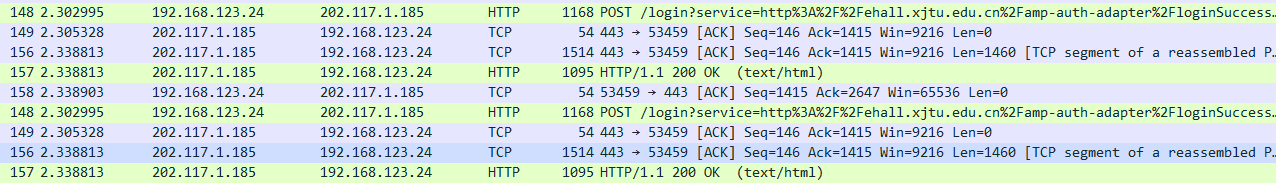
\includegraphics[width=12cm]{image/http-1}
	\caption{解密后分组(局部)}
	\label{fig12}
\end{figure}
\qquad
在解密之前,TLS应用数据层的内容是加密后的乱码,无法看到明文。通过上一小节对TLS握手过程的分析,得知这些内容是使用服务端提供的公钥加密的,因此客户端上应该保存有这份公钥,只要拿到这份公钥就可以对内容进行解密。事实上,一般的浏览器都会将TLS握手后得到的公钥保存在本地,通过设置环境变量可以改变公钥存放的位置,如图 \ref{fig13} 所示。然后在Wireshark菜单栏中依次点击“编辑->首选项->Protocol->SSL”,在出现的窗口中找到“(Pre)-Master-Secret log filename”下方的文本框,输入公钥保存的位置,如图 \ref{fig14} 所示。\\
\qquad
完成以上设置后再开始抓包。得到分组后,右键点击需要解密的分组,在弹出的菜单中点击“解码为...”,根据分组字段内容设置好相应的参数后即可完成解密。本实验中最终解密得到的客户端向服务端提交的登录表单的内容如图 \ref{fig15} 所示,表单中包含用户名、密码等信息。
\begin{figure}
	\centering
	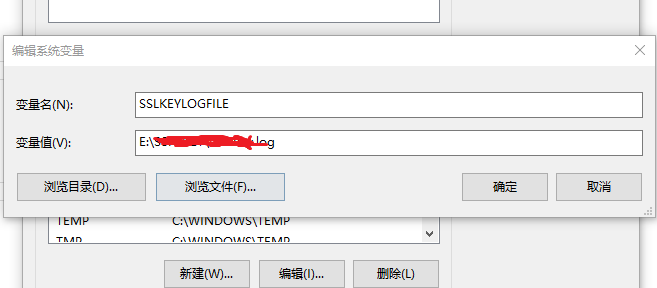
\includegraphics[width=12cm]{image/SSHKEY}
	\caption{通过设置环境变量改变浏览器保存公钥的位置}
	\label{fig13}
\end{figure}
\begin{figure}
	\centering
	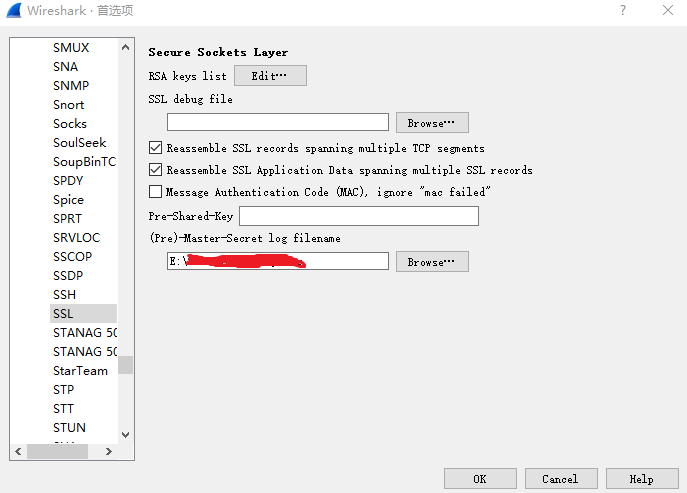
\includegraphics[width=12cm]{image/SSHKEY-1}
	\caption{在Wireshark中设置公钥保存位置}
	\label{fig14}
\end{figure}
\begin{figure}
	\centering
	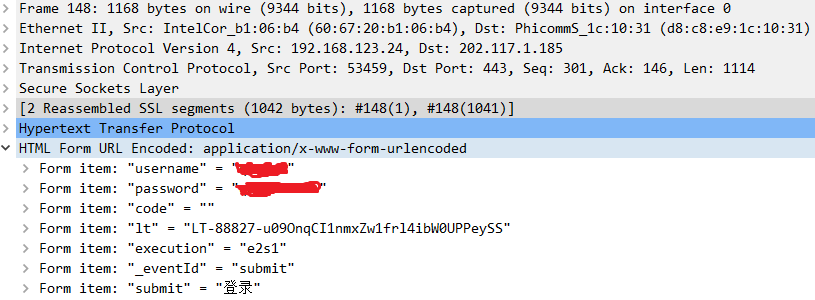
\includegraphics[width=12cm]{image/SSHKEY-2}
	\caption{解密后登录表单的内容}
	\label{fig15}
\end{figure}